\chapter{The Open Computing Abstraction Layer for Extended
Cellular Automata and the Finite Differences Method}

This chapter introduces OpenCAL, an open source computing
  abstraction layer defining a domain specific language for Extended
  Cellular Automata and the Finite Differences method (see chapters \ref{ch:CA} and \ref{ch:FDM} at page \pageref{ch:CA} and \pageref{ch:FDM} repectively). 
  Different implementations have been developed, which allow for transparent
  parallelism and are able to exploit multicore CPUs and manycore
  devices like GPUs, thanks to the adoption of OpenMP and OpenCL,
  respectively, as well as distributed memory architectures and/or multiple GPUs concurrently.
   System software architecture is presented and the
  underlying adopted data structures and algorithms are described in
  detail. Numerical correctness and efficiency have been assessed by
  considering the well known $SciddicaT$ Computational Fluid Dynamics
  landslide simulation model as reference example.  
  Moreover, a comprehensive study has been performed to device the best platform
  for execution as a function of numerical complexity and
  computational domain extent. Obtained results have highlighted the
  OpenCAL suitability for numerical models development and their execution on
  the most suitable high-performance parallel computational device.
  
\section{Introduction}
\label{sec:opencal_introduction}
 Scientific Computing \cite{golub2014scientific} is a broad and
  constantly growing multidisciplinary research field that uses formal
  paradigms to study complex problems and solve them through
  simulation by using advanced computing techniques and capabilities.
  
   Different formal paradigms have been proposed to provide the
  abstraction context in which problems are formalized. Partial
  Differential Equations (PDEs) were probably the first to be largely
  employed for describing a wide variety of phenomena. Unfortunately,
  PDEs can be analytically solved only for a small set of simplified
  problems \cite{Mazumder20161} and Numerical Methods have to be
  employed to obtain approximate solutions for real life applications. Among
  them, the Finite Differences Method (FDM) was one of the first
  considered, still currently employed, to address a wide variety of
  phenomena such as acoustics \cite{Chaigne19941112, Branski2014},
  heat \cite{Rana2012212, Sahin200619}, computational fluid dynamics
  (CFD) \cite{Chang1990317, Deng201390}, and quantum mechanics
  \cite{Hu2015640, Farrokhabadi201467} and many others.
  
  
  
Besides other solutions proposed for numerically approximating PDEs
  like, for instance, Finite Elements \cite{Hutton} and Finite Volume Methods \cite{Moukalled}, further formal paradigms were more recently proposed for modeling complex systems. Among them, Cellular Automata (CA) \cite{vonNeumann:1966:TSA:1102024} are Turing-equivalent \cite{Codd:1968:CA:1098682, Cook04a} parallel computational models. CA are widely studied from a theoretical point
  of view \cite{Wolfram-1984, Langton-1990b, Wolfram-2002,
    Ninagawa201542}, and their application domains vary from
  Artificial Life \cite{Langton-1986, Beer2004309} to Computational
  Fluid Dynamics \cite{Frish&al-1986, McNamara&Zanetti-1988,
    Higuera&Jimenez-1989, Aidun2010439}, besides many others. See chapter \ref{ch:CA} for an extensive introduction on Cellular Automata.
    
Regardless from the adopted formal paradigm, the simulation of
complex systems often requires the execution of a very large number of computer instruction and this explains why nowadays scientific computing is very oftern linked to  Parallel Computing. 

OpenMP is the  most widely adopted solution for parallel programming on shared
  memory computers \cite{Chapman:2007:UOP:1370966}. It fully supports
  parallel execution on multi-core CPUs and, starting from the 4.0
  release, also includes support of accelerators like graphic
  processing units (GPUs) or Xeon Phi co-processors. Unfortunately,
  compiler support for the $4.0$ release is quite recent and, in
  practice, current OpenMP applications mainly run on CPUs
  \cite{Oliverio2011271, Amritkar2014501, pop:hal-00786675}. However,
  in recent years, general purpose computing on graphic processing
  units (GPGPU), which exploits GPUs and many-core coprocessors for
  general purpose computation, has gained wide acceptance as an
  alternative solution for high-performance computing, resulting in a
  rapid spread of applications in many scientific and engineering
  fields \cite{Owens200780}. Most implementations are currently based
  on Nvidia CUDA (see e.g. \cite{Blecic2013, D'Ambrosio2013630,
    DiGregorio20131183, D'Ambrosio201230}), one of the first platforms
  proposed to exploit GPUs computational power on NVIDIA hardware. An
  open alternative to CUDA is OpenCL \cite{Stone201066}, an
  Application Program Inferface (API) originally proposed by Apple and
  currently managed by Khronos Group for parallel programming on
  heterogeneous devices like CPUs, GPUs, Digital Signal Processors
  (DSPs), and Field-Programmable Gate Arrays (FPGAs). Interest in
  OpenCL is continuously growing and many applications can already be
  found in literature \cite{Macri2015328, Bedorf20122825, Du2012391,
    Brown2011898}. However, an OpenCL parallelization of a scientific
  application is often a non-trivial task and, in many cases, requires
  a thorough refactorization of the source code. For this reason, many
  computational layers were proposed, which make many-core
  coprocessors computational power easier to be exploited. For
  instance, ArrayFire \cite{Malcolm2012} is a mathematical library for
  matrix-based computation such as linear algebra, reductions, and
  Fast Fourier transform; clSpMV \cite{Su2012353} is a sparse matrix
  vector multiplication library; clBlas \cite{clBlas-2016} is an
  OpenCL parallelization of the Blas linear algebra library. Examples
  of higher level computational layers, which provide the abstraction
  of formal computational paradigms, are OP2 \cite{Giles20131451},
  which is an open-source framework for the execution of unstructured
  grid applications on clusters of GPUs or multi-core CPUs, AQUAgpusph
  \cite{Cercos-Pita2015295}, which is a smoothed-particle
  hydrodynamics solver, and ASL \cite{asl}, an accelerated
  multiphysics simulation software based, among others, on the Lattice
  Boltzmann Method. Such high-level computational layers are briefly
  overviewed in the next section, together with some other significant
  examples.

This chapter is devoted to the description of OpenCAL which aims to be a portable parallel computing abstraction layer for scientific computing. OpenCAL is released under Lesser GNU Public Licence (LGPL) version 3 and is freely downloadable from GitHub at the following link: \url{https://github.com/OpenCALTeam/opencal}. OpenCAL allows for  the definition of computational models based on CA, XCA and FDM. It is designed to be easily extended and applied to all computational methods based on regular and uniform grids. 
The implementation descripted in this chapter targets shared multicore, distributed memory and GPUs and is designed to make the parallelism trqansparent to the user addressing and hiding many aspects of the underlying formal computational model and parallel execution platform. 

\subsection{An Overview on Scientific Simulation Software}
In this section, we present a non-exhaustive overview of some
  interesting and widely adopted parallel computing simulation software, which provide a
  high-level approach for the modeling of complex systems, hiding  low-level implementation issues such as memory allocation/de-allocation, thread management, and I/O  operations.General purpose simulation software,
  like Mathematica or Matlab, are intentionally not considered here.
\subsubsection{DEVS}
  DEVS \cite{Zeigler:1997:DEH:615253.615512, Zeigler:2000:TMS:580780},
  abbreviation of Discrete Event System Specification, is a modular
  and hierarchical formalism for modeling and analyzing general
  systems which can be described in terms of state transition
  tables. It also allows to describe continuous state systems (which
  can be formalized in terms of differential equations), and hybrid-
  continuous state and discrete event systems. The basic DEVS
  formalism allows to describe the inputs, outputs and states of a
  model (called atomic), besides the relationships among
  them. Furthermore, atomics can be used as building blocks for larger
  coupled models. Both atomic and coupled models adopt the same
  interface protocol, allowing to use a model as a component in
  another, larger model. Several extensions to the original DEVS
  formalism have been developed. Among these, P-DEVS
  \cite{Chow:1994:PDP:193201.194336} is a modeling formalism which
  provides both conceptual and parallel execution benefits with
  respect to the original DEVS formalism, while Cell-DEVS
  \cite{Wainer:2009:DMS:1611320} is an extension of the DEVS formalism
  that allows the definition of Cellular Automata models. A wide
  variety of models have been developed using this approach, such as
  fire spreading models with different conditions, formation of a
  watershed and robots in a manufacturing plant
  \cite{Troccoli:2001:MCP:882496.884491}.
\subsubsection{OP2}
  OP2 \cite{Giles20131451} is an open-source framework for the
  execution of unstructured grid applications on clusters of GPUs or
  multi-core CPUs. The main characteristic of the library is the use
  of source-to-source translation to generate efficient back-end code
  for state-of-the-art hardware for the different target
  platforms. Specifically, OP2 aims to separate the scientific
  specification of an application from its parallel implementation to
  achieve code endurance and near-optimal performance by re-targeting
  the back-end to different multi-core/many-core hardware. The OP2
  \emph{active} library approach uses program transformation tools, so
  that a single application code written using the OP2 API is
  transformed into the appropriate form that can be linked against a
  target parallel implementation (e.g. OpenMP, CUDA, OpenCL, MPI,
  etc.) enabling execution on different back-end hardware
  platforms. In order to facilitate the development of unstructured
  mesh applications at a higher hardware agnostic level, OP2 provides
  both a C/C++ and a Fortran API. This enables application developers
  to focus on solving problems at a higher level and not worry about
  architecture specific optimisations. As a consequence, the problem
  domain space can be separated into both a higher application level
  to concentrate on solving domain specific problems and write code
  that remains unchanged for different underlying hardware, and in the
  meanwhile consider a lower implementation level, that focuses on how
  a computation can be executed most efficiently on a given platform
  by carefully analysing the data access patterns.  The performance
  impact of the library design choices have been quantified on a range
  of NVIDIA GPUs using the end-to-end performance of an industrial
  representative CFD application (Airfoil) developed using the OP2
  API. The full OP2 source, the Airfoil test case code and the
  auto-tuning framework are available as open source software
  \cite{OP2Web}.
\subsubsection{CAMELot}
  CAMELot \cite{dattilo2003simulation, Mendicino2006, d2007parallel}
  is a proprietary CA and XCA high performance simulation environment
  derived from CAMEL \cite{cannataro1995parallel}. The system supports
  CARPET, a purpose-built language for CA programming based on C with
  additional constructs to describe the rule of the state transition
  function of a single cell of a cellular automaton and, eventually, to steer the
  application. Specifically, a CARPET program is composed of a declaration part that
  describes the properties of CA (dimension, radius, state, neighbour,
  parameters, region), a body program that implements the transition
  function, and a steering part that contains a set of commands for
  extracting and analysing system information and performing
  computational steering (i.e., global operations). The steering
  section is performed by the runtime system at each iteration, after
  the transition functions of all cells have been evaluated.  The
  state of a cell is defined as a record of typed \emph{substates}
  (char, shorts, integers, floats, doubles and one-dimensional
  arrays), and even complex neighbourhoods (e.g., hexagonal, Margolus)
  can be simply defined by means of a CARPET
  statement. Non-deterministic, time-dependent and non-uniform
  transition functions can also be defined. Camelot offers an
  integrated programming environment, an interactive user interface
  and permits the efficient and seamless simulation of XCA on
  distributed memory computers.
\subsubsection{libAuToti}
  An open-source alternative to CAMELot is libAuToti
  \cite{spingola2008modeling}, an efficient and flexible parallel XCA
  library. Similarly to CAMELot, libAuToti allows for a simple and
  concise definition of both the transition function and the other
  characteristics of XCA model definition. It allows for both
  sequential and parallel execution, both on shared and distributed
  memory machines (thanks to the adoption of the Message Passing
  paradigm for the interprocesses communications), by hiding parallel
  implementation issues to the user. The library also implements a
  dynamic load balancing algorithm to better exploit computational
  resources and reduce overall execution time
  \cite{DBLP:conf/csc/ZitoDSSRA09}. A multithread version was also
  developed to better exploit multi-core architectures, coupled with
  an interactive 2D/3D visualization system based on VTK
  \cite{spataro2010multithread}.
\subsubsection{ASL}
  The Advanced Simulation Library (ASL) \cite{asl} is a free and open
  source hardware accelerated multiphysics simulation software. It is
  based, among others, on the Lattice Boltzmann Method and is written
  in OpenCL, which enable efficient deployment on a variety of
  massively parallel architectures. However, no OpenCL knowledge is
  strictly required to develop ASL-based applications, thanks to a
  simplified C++ API. ASL can be used to model various coupled
  physical and chemical phenomena and employed in a multitude of
  fields like computational fluid dynamics, computer-aided
  engineering, and crystallography.  Mesh-free, immersed boundary
  approach allows to move from CAD directly to computations
  eliminating pre-processing efforts and reducing amount of potential
  errors.
\subsubsection{AQUAgpusph}
  Eventually, AQUAgpusph \cite{CercosPita2015295} is a free Smoothed
  Particle Hydrodynamics (SPH - a mesh-free Lagrangian method to solve
  Navier-Stokes equations) software accelerated with OpenCL. The main
  advantages with respect to other existing SPH libraries are the use
  of OpenCL instead of CUDA, which allows for parallel execution on a
  variety of massively parallel devices, the implementation of the
  most popular boundary conditions, the easy customization of the code
  to different problems, the extensibility with regard to Python
  scripts and the runtime output which allows the tracking of
  simulations in real time, or a higher frequency in saving some
  results without a significant performance lost. Authors have proven
  to improve the solver speed, the results quality, and the usability
  for a wider areas of application.
  
  \section{OpenCAL Software Architecture and the Considered Parallel Computing Paradigms}
  This section describes the software architecture of the first
  OpenCAL release. As described in Figure \ref{fig:architecture}, a
  computational model can be designed at the higher level of
  abstraction. As already stated, supported computational paradigms
  are CA, XCA and FDM. At this level, the main features of the
  computational model like dimensions, neighborhood, boundary
  conditions, involved substates and elementary processes, are
  designed. The simulation process, which allows to obtain the model
  evolution at discrete time steps, is also defined at this level, by
  specifying the initial condition of the system, global operations
  (like steering or global reductions), the initial and final
  computational step and a possible stopping criterion. Eventually,
  optimizations can be considered, namely the explicit update, which
  allows to selectively update substates after the application of each
  elementary process, and the quantization feature, which allows to
  restrict the computation to a subset of the computational domain, by
  excluding stationary cells.
  
  \begin{figure}[H]
  \begin{center}
    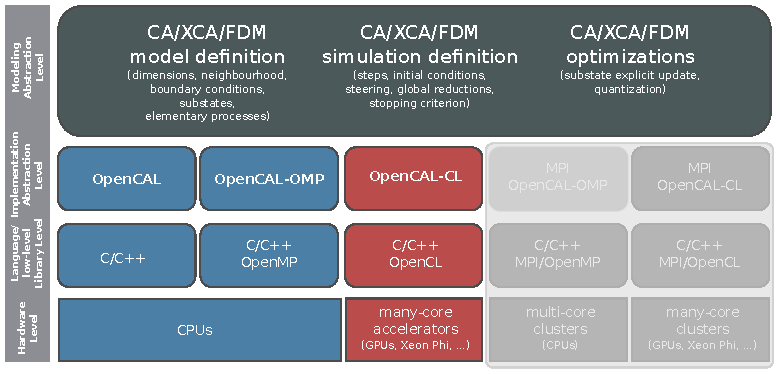
\includegraphics{./artworks/Figure05.pdf}
    \caption{}
    \label{fig:architecture}
  \end{center}
\end{figure}
  
   OpenCAL can be found in the implementation abstraction level. As it
  can be seen, four different versions can be considered for
  implementing the previously designed computational model, namely
  OpenCAL, OpenCAL-OMP and OpenCAL-CL and OpenCAL-MPI. The first one refers to the   serial implementation of the library, while second and the third are OpenMP  and OpenCL-based parallelizations, respectively, as pointed out by
  the language/low-level library level. The fourth one is a cluster ready implementation that allows to execution on distributed memory cluster where each node can exploit multiple GPUs.
  All implementations are written in C for the maximum efficiency and provide high-level data types and functions that match the XCA formal components, allowing  for a straightforward implementation of the designed computational
  model, by also allowing to ignore low-level issues like memory
  management and I/O operations. In this respect, OpenCAL can be
  considered as a domain-specific language (DSL) for the CA, XCA and
  FDM computational methods. Finally, at the hardware level, depending
  on the adopted version of the library, execution can be performed on
  single- and multi-core CPUs, or on many-core accelerators like GPUs,
  almost transparently to the user.